The domain adaptation in imitation learning can be formalized as a Markov decision problem which was introduced in Chapter~\ref{ch:Background}.
As a brief reminder,
an episodic Markov Decision Process (MDP) $\mathbb{M}$ with finite time horizon $H$ \cite{RL_AnIntroductionBook} is represented as the following equation:

\[
  \mathbb{M} = (\mathcal{S}, \mathcal{A}, P, R, \gamma, H)
\]

where
$\mathcal{S}$ and $\mathcal{A}$
represent the state and action spaces,
respectively;
$P(s'|s, a)$ denotes the transition function,
$R: \mathcal{S} \times \mathcal{A} \to \mathbb{R}$ is the reward function,
$\gamma$ is the discount factor---whereas,
a policy $\pi(s|a): \mathcal{S} \to \mathcal{A}$ for $\mathbb{M}$
describes a mapping from states $\mathcal{S}$ to actions $\mathcal{A}$.

It should be noted that in the domain adaptive imitation learning setting,
the reward function is not given beforehand.
Therefore,
the MDP for a domain $x$ without reward is defined as
$\mathbb{M}^-_x = (\mathcal{S}_x, \mathcal{A}_x, P_x, \gamma_x, H_x)$.
All examined domains are assumed to be alignable.
That is, if considering two domains $x$ and $y$, $\mathbb{M}^-_x$ can be reduced to $\mathbb{M}^-_y$,
denoted as $\mathbb{M}^-_x \ge \mathbb{M}^-_y$, or vice versa \cite{DAIL_Model_DAIL}.
An example is illustrated in Figure \ref{ch:DAIL:fig:MDP_Reduction}.
Based on this expression,
let $\mathcal{E}$ and $\mathcal{L}$ be the expert and the learner (agent) domain,
respectively,
$\mathbb{M}^-_\mathcal{E}$ and $\mathbb{M}^-_\mathcal{L}$ are said to be alignable if and only if $\mathbb{M}^-_\mathcal{E} \ge \mathbb{M}^-_\mathcal{L}$ or $\mathbb{M}^-_\mathcal{L} \ge \mathbb{M}^-_\mathcal{E}$ \cite{DAIL_Model_DAIL}.

Furthermore, $\tau_{x} = \{(s^t_{x}, a^t_{x}) : t \in [0, \mathcal{H}]\}$ denotes a demonstration in the domain $x$,
which is a sequence of state--action pairs.
Then, a set of demonstrations
$\mathcal{D}_\mathcal{E}=\{\tau^i_\mathcal{E} : i\in[1,N]\}$ from $\mathcal{E}$ is assumed to be available at the training time.
With those assumptions,
the main objective is being able to learn an optimal learner domain policy $\pi^{*}_\mathcal{L}$ against unknown reward functions $\mathcal{R}_\mathcal{E}$ and $\mathcal{R}_\mathcal{L}$, given the expert demonstrations $\mathcal{D}_{\mathcal{E}}$.

\begin{figure}[htbp!]
  \centering
  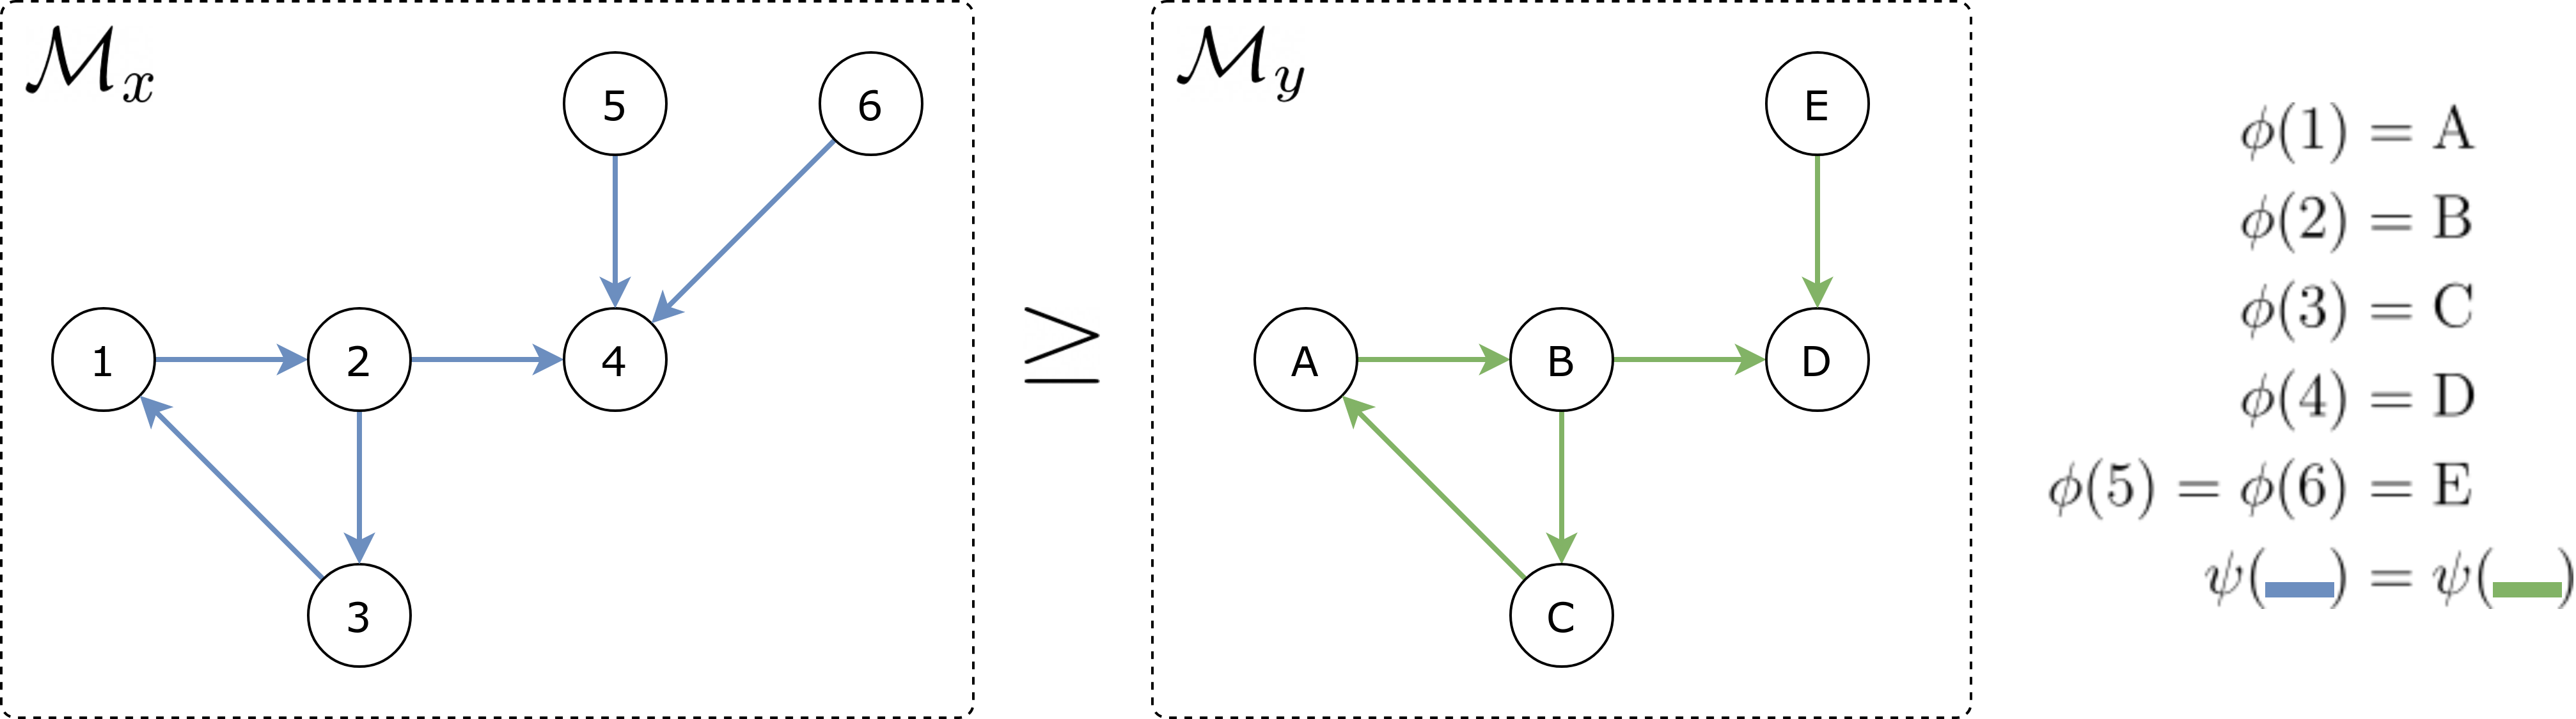
\includegraphics[width=0.9\linewidth]{\FigsDir/MDP_Reduction.png}
  \caption{An example of two MDPs for $x$ and $y$ domains where $\mathbb{M}_x \ge \mathbb{M}_y$. $\phi: \mathcal{S}_x \to \mathcal{S}_y$ and $\psi: \mathcal{A}_x \to \mathcal{A}_y$ are state and actions maps, respectively. States correspond to nodes and actions to colors. States 5, 6 in $\mathcal{S}_x$ are merged to state $e$ in $\mathcal{S}_y$ and blue actions in $\mathcal{A}_x$ are mapped to green actions in $\mathcal{A}_y$.}
  \label{ch:DAIL:fig:MDP_Reduction}
\end{figure}
